\documentclass[12pt,a4paper]{article}
\usepackage[utf8]{inputenc}
\usepackage{cmap}
\usepackage[T2A]{fontenc}
\usepackage[russian]{babel}
\usepackage{graphicx}
\usepackage{booktabs}
\usepackage{longtable}
\usepackage{geometry}
\usepackage{float}
\geometry{top=2cm, left=2cm, right=2cm, bottom=2cm}
\usepackage{paracol}
\usepackage{src/title}
\usepackage{hyperref}
\usepackage{listings}
\usepackage{xcolor}
\usepackage{pgfplots}
\pgfplotsset{compat=1.18}

\title{Лабораторная работа №5. Дерево решений для классификации грибов}
\author{Ануфриев А.С. 465029}
\supervisor{Болдырева Елена Александровна}
\date{08.11.2026}

\abstract{Построено небинарное дерево решений для бинарной классификации грибов (съедобный / ядовитый) на датасете UCI Mushroom без использования сторонних библиотек для построения дерева и оценки качества. Отобраны случайным образом $\sqrt{n}$ признаков, реализованы метрики Accuracy, precision, recall и кривые AUC-ROC и AUC-PR. Приведены результаты на тестовой выборке.}
\keywords{дерево решений, бинарная классификация, грибы, AUC-ROC, AUC-PR, Python, NumPy}

\begin{document}
\maketitle

\section{Цель и задачи работы}
Целью работы является реализация алгоритма построения дерева решений для задачи бинарной классификации грибов (съедобный / ядовитый) на датасете UCI Mushroom и оценка его качества. Основные этапы:
\begin{enumerate}
\item загрузка и предобработка исходных данных;
\item случайный отбор $\sqrt{n}$ признаков;
\item построение небинарного дерева решений собственным кодом без сторонних библиотек для построения дерева;
\item оценка по Accuracy, precision и recall без использования библиотек;
\item построение кривых AUC-ROC и AUC-PR без использования библиотек.
\end{enumerate}

\section{Исходные данные}
Используется датасет UCI Mushroom с классификацией грибов (файл \emph{agaricus-lepiota.data}; семейства \textit{Agaricus} и \textit{Lepiota}, источник --- справочник \emph{The Audubon Society Field Guide to North American Mushrooms}, 1981). Датасет содержит 8124 объекта, каждый описывается классом (съедобный \texttt{e} / ядовитый \texttt{p}) и 22 номинативными признаками (форма шляпки, запах, цвет спорового порошка и т.д.). Все признаки имеют дискретное множество значений; пропуски обозначены ``?'', встречаются только в признаке ``stalk-root''.

После удаления объектов с пропусками остаётся 5644 записи: 3488 съедобных (61.8\%) и 2156 ядовитых (38.2\%).

\section{Метод: дерево решений}
Построение дерева выполняется рекурсивно сверху вниз (подход алгоритма C4.5). В каждом узле выбирается признак с максимальным нормированным приростом информации:
\[
\mathrm{GainRatio}(X) = \frac{\mathrm{Info}(T) - \mathrm{Info}_X(T)}{\mathrm{splitinfo}(X)},
\]
где $\mathrm{Info}(T) = -\sum_{j} p_j \log_2 p_j$ --- энтропия множества примеров $T$, $\mathrm{Info}_X(T) = \sum_i \frac{|T_i|}{|T|}\mathrm{Info}(T_i)$ --- условная энтропия после разбиения по признаку $X$, $\mathrm{splitinfo}(X) = -\sum_i \frac{|T_i|}{|T|}\log_2\frac{|T_i|}{|T|}$. По выбранному признаку создаются столько потомков, сколько у него значений (дерево не бинарное). Рекурсия продолжается до исчерпания примеров в узле, достижения максимальной глубины или нулевого прироста информации. Лист получает класс большинства объектов в узле. Дерево реализовано через класс узла со ссылками на потомков (список-списков не используется).

\section{Ход работы}
\begin{enumerate}
\item Чтение исходных данных; исключение записей с пропущенными значениями в признаке ``stalk-root''.
\item Случайный отбор $\sqrt{22} \approx 4$ признаков с фиксированным зерном генератора: \emph{cap-shape}, \emph{cap-surface}, \emph{gill-color}, \emph{stalk-color-above-ring}.
\item Стратифицированное разделение на обучающую (70\%) и тестовую (30\%) выборки: 3951 и 1693 объекта соответственно, соотношение классов сохранено.
\item Построение дерева на обучающей выборке: глубина 4, 85 внутренних узлов, 63 листа.
\item Получение меток классов и вероятностей (доля ядовитых в листе) для объектов тестовой выборки.
\item Расчёт Accuracy, precision, recall, построение кривых AUC-ROC и AUC-PR собственным кодом без библиотек.
\end{enumerate}

\section{Результаты}
Таблица~\ref{tab:metrics} содержит элементы матрицы ошибок и качество классификации на тестовой выборке (положительный класс --- ядовитый гриб).

\begin{table}[H]
\centering
\caption{Матрица ошибок и метрики качества на тестовой выборке (1693 объекта).}
\label{tab:metrics}
\begin{tabular}{lrrr}
\toprule
 & Значение & & \\
\hline
TP (яды распознаны) & 472 & FP (съедобные как яды) & 71 \\
TN (съедобные распознаны) & 975 & FN (яды как съедобные) & 175 \\
\midrule
Accuracy & \multicolumn{3}{r}{0.8547} \\
Precision & \multicolumn{3}{r}{0.8692} \\
Recall & \multicolumn{3}{r}{0.7295} \\
AUC-ROC & \multicolumn{3}{r}{0.9416} \\
AUC-PR & \multicolumn{3}{r}{0.9223} \\
\bottomrule
\end{tabular}
\end{table}

Дерево даёт высокую точность (85.5\%) и высокую AUC-ROC (0.9416). При этом recall 0.7295 означает, что часть ядовитых грибов классифицируется как съедобные, что для задачи безопасного потребления является ограничением.

\begin{figure}[H]
\centering
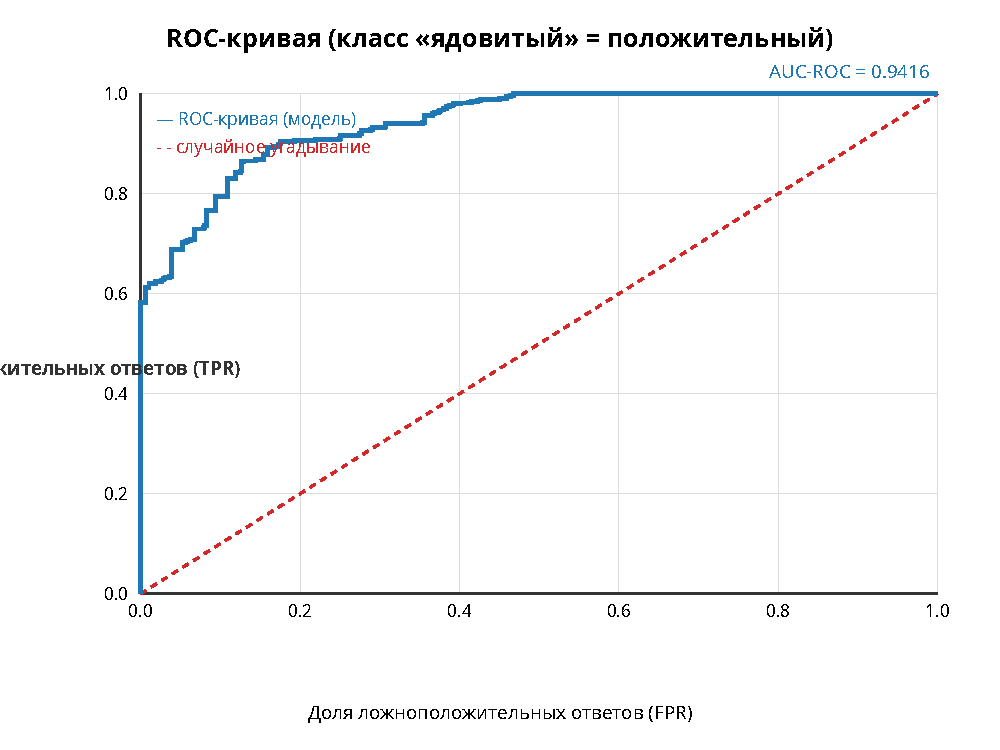
\includegraphics[width=0.48\textwidth]{../graphics/roc_plot.pdf}
\quad
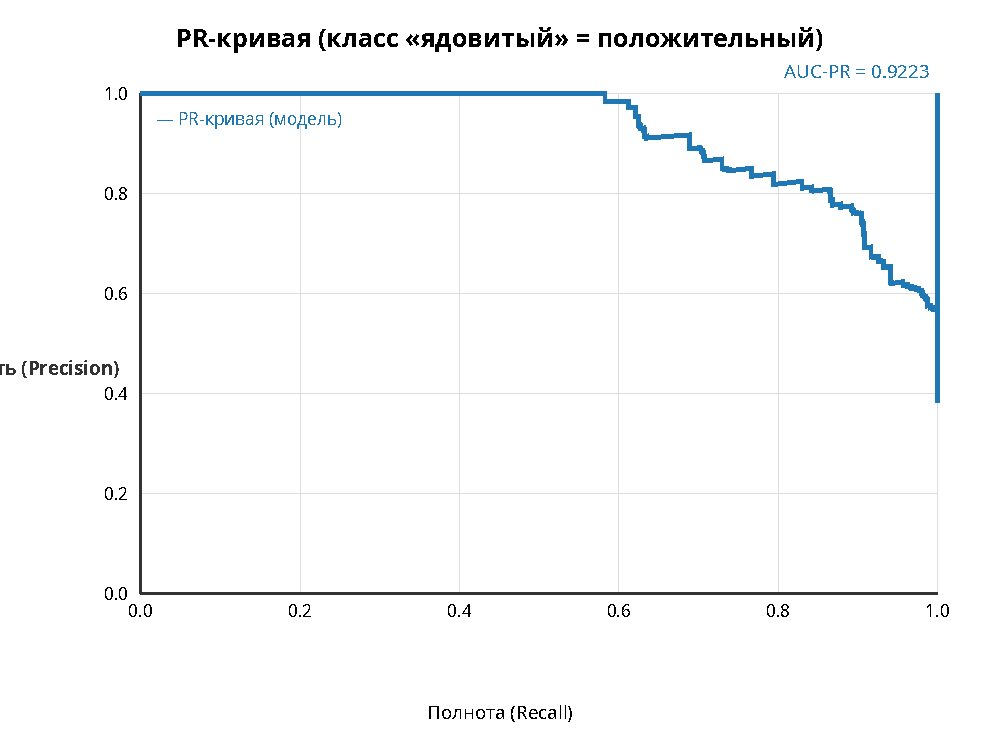
\includegraphics[width=0.48\textwidth]{../graphics/pr_plot.pdf}
\caption{Контрольные кривые качества классификатора на тестовой выборке: ROC-кривая (AUC-ROC = 0.9416) и PR-кривая (AUC-PR = 0.9223). Построены из фактических данных тестовой выборки.}
\end{figure}

\section{Выводы}
Реализовано небинарное дерево решений для бинарной классификации грибов без сторонних библиотек. На отобранных случайным образом 4 признаках дерево глубины 4 достигает Accuracy 0.8547, precision 0.8692 и recall 0.7295 на тестовой выборке; AUC-ROC = 0.9416, AUC-PR = 0.9223. Получение вероятностей классов из долей объектов в листьях позволяет построить ROC- и PR-кривые и компактно оценить всю область порогов принятия решений.

\section{Список литературы}
\begin{enumerate}
\item Schlimmer, J.C. (1987). Concept Acquisition Through Representational Adjustment. Technical Report 87-19, Department of Information and Computer Science, University of California, Irvine. (Donor of the UCI Mushroom dataset.)
\item Aha, D.W. (1988). Comments on the Mushroom Database. University of California, Irvine.
\item Quinlan, J.R. (1993). C4.5: Programs for Machine Learning. Morgan Kaufmann, San Mateo, CA.
\item Lincoff, G.H. (1981). The Audubon Society Field Guide to North American Mushrooms. Alfred A. Knopf, New York.
\end{enumerate}

\section{Приложение}
Исходные параметры эксперимента: фиксированное зерно генератора 42; отбор $\sqrt{n}$ признаков (4 из 22); стратифицированное разбиение 70/30; критерий разбиения --- нормированный прирост информации (C4.5); максимальная глубина 12 (достигнута 4); остановка при чистом узле, отсутствии прироста или исчерпании признаков. Реализация выполнена на Python с использованием NumPy; построение дерева, расчёт метрик и кривых выполнены собственным кодом без сторонних библиотек.

Положительный класс в дальнейшем --- ядовитый гриб (\texttt{p}); отрицательный --- съедобный (\texttt{e}).

Расчёт кривых AUC-ROC и AUC-PR: объекты тестовой выборки сортируются по убыванию оценки вероятности класса ``ядовитый'' (доля таких объектов в листе дерева). При каждом пороге вычисляются $TPR = TP/(TP+FN)$, $FPR = FP/(FP+TN)$ --- точки ROC-кривой, и $Precision = TP/(TP+FP)$, $Recall = TP/(TP+FN)$ --- точки PR-кривой. Площадь под кривыми считается методом трапеций по отсортированным точкам; начальные точки $(0,0)$ и $(1,1)$ (ROC) и $(0,1)$ (PR) добавляются явно. Все расчёты --- собственные, без библиотек.

Таблица~\ref{tab:thresholds} содержит точки работы классификатора (порог вероятности, FPR, TPR, precision, recall) при всех distintos значениях вероятности на тестовой выборке; по ним можно воспроизвести значения AUC-ROC $= 0.9416$ и AUC-PR $= 0.9223$.

\begin{table}[H]
\centering
\caption{Точки работы классификатора по порогам вероятности класса «ядовитый» (тестовая выборка, 1693 объекта).}
\label{tab:thresholds}
\begin{tabular}{ccccc}
\toprule
Порог & FPR & TPR & Precision & Recall \\
\midrule
1.000000 & 0.000000 & 0.582689 & 1.000000 & 0.582689 \\
0.782609 & 0.010516 & 0.621329 & 0.973366 & 0.621329 \\
0.600000 & 0.041109 & 0.689335 & 0.912065 & 0.689335 \\
0.534884 & 0.067878 & 0.729521 & 0.869245 & 0.729521 \\
0.461538 & 0.083174 & 0.766615 & 0.850772 & 0.766615 \\
0.438596 & 0.108987 & 0.829985 & 0.824885 & 0.829985 \\
0.432432 & 0.119503 & 0.842349 & 0.813433 & 0.842349 \\
0.344444 & 0.153920 & 0.877898 & 0.779150 & 0.877898 \\
0.333333 & 0.159656 & 0.891808 & 0.775538 & 0.891808 \\
0.277778 & 0.178776 & 0.904173 & 0.757772 & 0.904173 \\
0.240000 & 0.191205 & 0.904173 & 0.745223 & 0.904173 \\
0.220588 & 0.224665 & 0.908810 & 0.714459 & 0.908810 \\
0.206522 & 0.250478 & 0.916538 & 0.693567 & 0.916538 \\
0.196078 & 0.318356 & 0.941267 & 0.646497 & 0.941267 \\
0.189189 & 0.356597 & 0.956723 & 0.623992 & 0.956723 \\
0.180000 & 0.380497 & 0.969088 & 0.611707 & 0.969088 \\
0.171717 & 0.380497 & 0.970634 & 0.612086 & 0.970634 \\
0.150000 & 0.411090 & 0.981453 & 0.596244 & 0.981453 \\
0.137931 & 0.450287 & 0.987635 & 0.575676 & 0.987635 \\
0.000000 & 1.000000 & 1.000000 & 0.382162 & 1.000000 \\
\bottomrule
\end{tabular}
\end{table}

Остановка рекурсии дерева: все объекты в узле одного класса, нулевой прирост информации, исчерпание признаков или достижение максимальной глубины 12 (фактическая глубина построенного дерева --- 4).
\end{document}

\end{document}
